%!TEX root = ../thesis.tex

\section{ROS}

ROS(Robot Operating System)は,オープンソースのロボットソフトウェアフレームワークで,ロボットアプリケーションの開発や実行をサポートするミドルウェアである.異なるバージョンが存在しているが,本研究ではROS Noeticを対象としている.

\subsection{LiDAR}

  LiDAR(Light Detection and Ranging)は,光を利用して距離を測定する技術で,具体的には,レーザー光を発射し,対象物に当たって反射し戻ってくるまでの時間を計測することで,距離を推定する.また,使用する装置によっては,物体によってどれだけの光が反射されたかを示す反射強度も測定することができる.したがって,LiDARは周囲の状況を把握し,環境認識や物体検知などに利用される.

  本研究で使用する2DLiDARを\figref{Fig:hokuyo_lidar}に示す.これは,北陽電気社製の2DLiDARであり,ROS上で\texttt{urg\_node}\cite{urg_node}というパッケージが提供されている.この\texttt{urg\_node}は,検出範囲(最大270 \,[deg])や反射強度の使用有無などのパラメータを変更するだけで簡単にデータのやり取りが可能である.

  \begin{figure}[h]
    \centering
    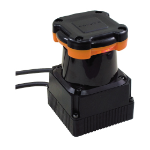
\includegraphics[keepaspectratio, scale=0.80] {images/RobotGuidance_hokuyo_lidar.png}
    \caption{Hokuyo 2DLiDAR (UTM-30LX) \cite{hokuyo}}
    \label{Fig:hokuyo_lidar}
  \end{figure}

\newpage

\subsection{RViz}

  RViz(ROS Visualization)\cite{rviz}は,ROSで提供される三次元ビジュアライゼーションツールであり,数値で表されるロボットの座標や各センサのデータ直感的に理解できる三次元空間上に表示することができる.\figref{Fig:RobotGuidance_rviz}にその様子を示す.ここでは,ロボットのモデルと2DLiDARからのセンサデータ,カメラ画像をリアルタイムに表示している.

  \begin{figure}[h]
    \centering
    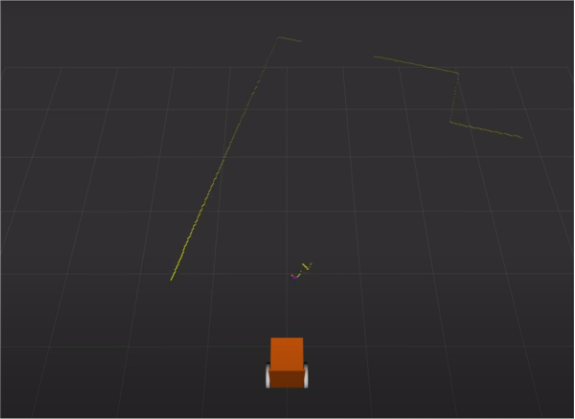
\includegraphics[keepaspectratio, scale=0.60] {images/RobotGuidance_rviz.png}
    \caption{RViz(Display robot model and scan data)}
    \label{Fig:RobotGuidance_rviz}
  \end{figure}

\newpage